\section{Numerical approximations}

\begin{figure}[h]
  \centering
  \caption{The graphs of numerical approximations of the solution curve for $b = 14$, $\sigma = \frac{1}{6}$ and $\rho = \frac{1}{16}$.}
  \subfloat[$a = 5$]{%
    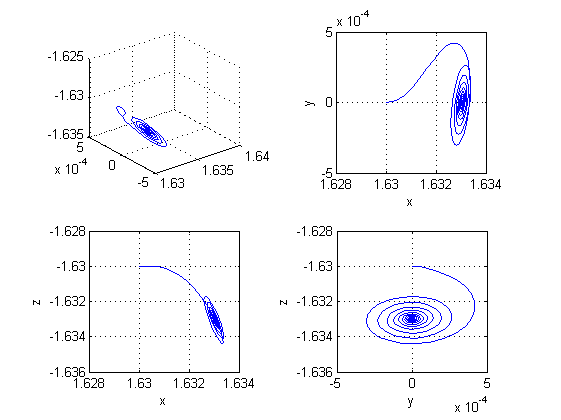
\includegraphics[width=0.5\textwidth]{a5.png}%
  }
  \subfloat[$a = 6.3$]{%
    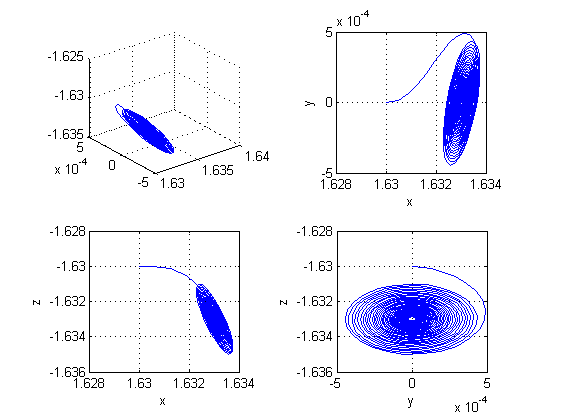
\includegraphics[width=0.5\textwidth]{a6-3.png}%
  }\\
  \subfloat[$a = 6.68$]{%
    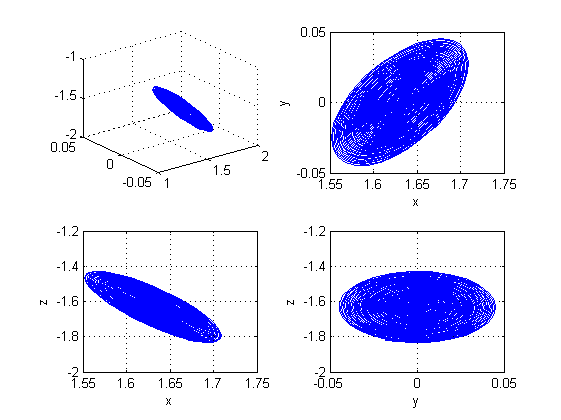
\includegraphics[width=0.5\textwidth]{a6-68.png}%
  }
  \subfloat[$a = 7.5$]{%
    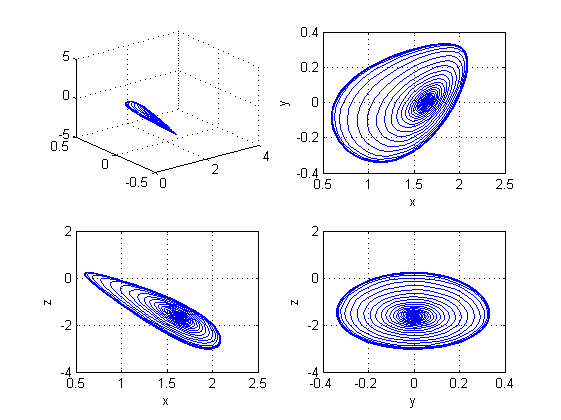
\includegraphics[width=0.5\textwidth]{a7-5.png}%
  }
  \label{fig:numapprox}
\end{figure}
\begin{figure}[h]
  \ContinuedFloat
  \centering
  \subfloat[$a = 8.5$]{%
    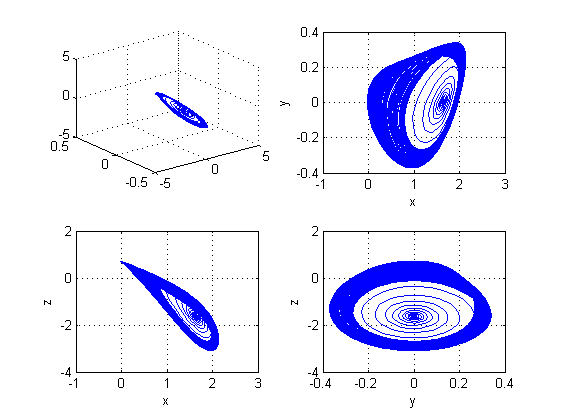
\includegraphics[width=0.5\textwidth]{a8-5.png}%
  }
  \subfloat[$a = 9$]{%
    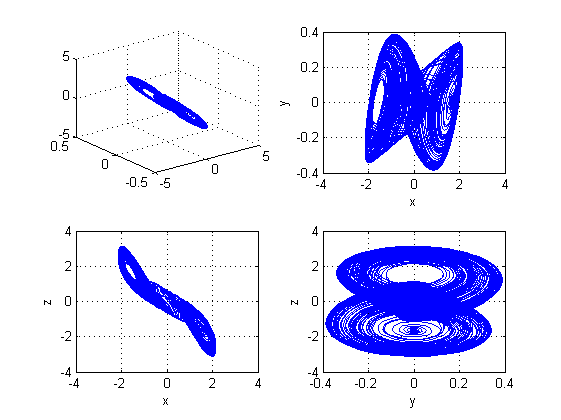
\includegraphics[width=0.5\textwidth]{a9.png}%
  }\\
  \subfloat[$a = 9.8$]{%
    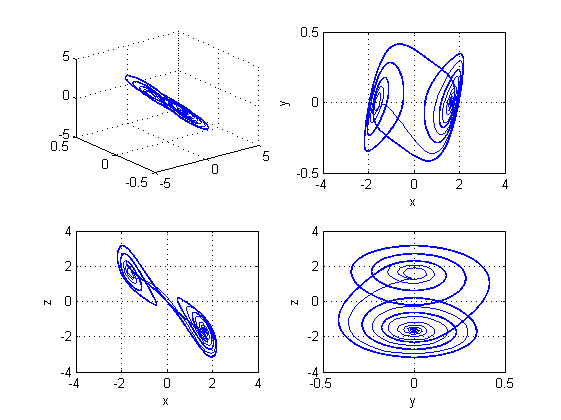
\includegraphics[width=0.5\textwidth]{a9-8.png}%
  }
  \subfloat[$a = 10.5$]{%
    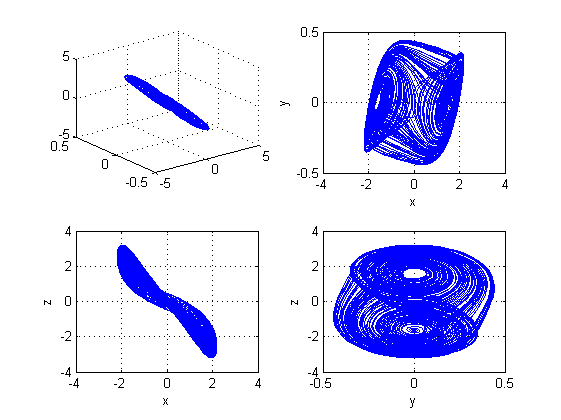
\includegraphics[width=0.5\textwidth]{a10-5.png}%
  }\\
  \subfloat[$a = 12$]{%
    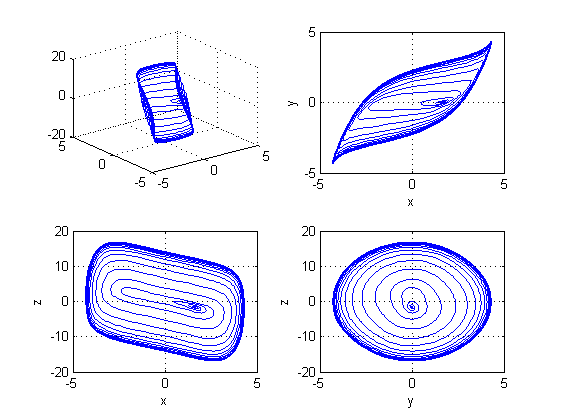
\includegraphics[width=0.5\textwidth]{a12.png}%
  }
\end{figure}

%%% Local Variables: 
%%% mode: latex
%%% TeX-master: "chua_circuit"
%%% End: 
